\documentclass[journal,12pt,twocolumn]{IEEEtran}

\usepackage[utf8]{inputenc}
\usepackage{kvmap}
\usepackage{graphics} 

\usepackage{setspace}
\usepackage{gensymb}

\singlespacing

\usepackage{amsthm}

\usepackage{mathrsfs}
\usepackage{txfonts}
\usepackage{stfloats}
\usepackage{bm}
\usepackage{cite}
\usepackage{cases}
\usepackage{subfig}

\usepackage{longtable}
\usepackage{multirow}

\usepackage{enumitem}
\usepackage{mathtools}
\usepackage{steinmetz}
\usepackage{tikz}
\usepackage{circuitikz}
\usepackage{verbatim}
\usepackage{tfrupee}
\usepackage[breaklinks=true]{hyperref}
\usepackage{graphicx}
\usepackage{tkz-euclide}
\usepackage{float}

\usetikzlibrary{calc,math}
\usepackage{listings}
    \usepackage{color}                                            %%
    \usepackage{array}                                            %%
    \usepackage{longtable}                                        %%
    \usepackage{calc}                                             %%
    \usepackage{multirow}                                         %%
    \usepackage{hhline}                                           %%
    \usepackage{ifthen}                                           %%
    \usepackage{lscape}     
\usepackage{multicol}
\usepackage{chngcntr}

\DeclareMathOperator*{\Res}{Res}

\renewcommand\thesection{\arabic{section}}
\renewcommand\thesubsection{\thesection.\arabic{subsection}}
\renewcommand\thesubsubsection{\thesubsection.\arabic{subsubsection}}

\renewcommand\thesectiondis{\arabic{section}}
\renewcommand\thesubsectiondis{\thesectiondis.\arabic{subsection}}
\renewcommand\thesubsubsectiondis{\thesubsectiondis.\arabic{subsubsection}}

\hyphenation{op-tical net-works semi-conduc-tor}
\def\inputGnumericTable{}                                 %%

\lstset{
%language=C,
frame=single, 
breaklines=true,
columns=fullflexible
}
\begin{document}

\newtheorem{theorem}{Theorem}[section]
\newtheorem{problem}{Problem}
\newtheorem{proposition}{Proposition}[section]
\newtheorem{lemma}{Lemma}[section]
\newtheorem{corollary}[theorem]{Corollary}
\newtheorem{example}{Example}[section]
\newtheorem{definition}[problem]{Definition}

\newcommand{\BEQA}{\begin{eqnarray}}
\newcommand{\EEQA}{\end{eqnarray}}
\newcommand{\define}{\stackrel{\triangle}{=}}
\newcommand\hlight[1]{\tikz[overlay, remember picture,baseline=-\the\dimexpr\fontdimen22\textfont2\relax]\node[rectangle,fill=blue!50,rounded corners,fill opacity = 0.2,draw,thick,text opacity =1] {$#1$};}
\bibliographystyle{IEEEtran}
\providecommand{\mbf}{\mathbf}
\providecommand{\pr}[1]{\ensuremath{\Pr\left(#1\right)}}
\providecommand{\qfunc}[1]{\ensuremath{Q\left(#1\right)}}
\providecommand{\sbrak}[1]{\ensuremath{{}\left[#1\right]}}
\providecommand{\lsbrak}[1]{\ensuremath{{}\left[#1\right.}}
\providecommand{\rsbrak}[1]{\ensuremath{{}\left.#1\right]}}
\providecommand{\brak}[1]{\ensuremath{\left(#1\right)}}
\providecommand{\lbrak}[1]{\ensuremath{\left(#1\right.}}
\providecommand{\rbrak}[1]{\ensuremath{\left.#1\right)}}
\providecommand{\cbrak}[1]{\ensuremath{\left\{#1\right\}}}
\providecommand{\lcbrak}[1]{\ensuremath{\left\{#1\right.}}
\providecommand{\rcbrak}[1]{\ensuremath{\left.#1\right\}}}
\theoremstyle{remark}
\newtheorem{rem}{Remark}
\newcommand{\sgn}{\mathop{\mathrm{sgn}}}
\providecommand{\abs}[1]{\left\vert#1\right\vert}
\providecommand{\res}[1]{\Res\displaylimits_{#1}} 
\providecommand{\norm}[1]{$\left\lVert#1\right\rVert$}
%\providecommand{\norm}[1]{\lVert#1\rVert}
\providecommand{\mtx}[1]{\mathbf{#1}}
\providecommand{\mean}[1]{E\left[ #1 \right]}
\providecommand{\fourier}{\overset{\mathcal{F}}{ \rightleftharpoons}}
%\providecommand{\hilbert}{\overset{\mathcal{H}}{ \rightleftharpoons}}
\providecommand{\system}{\overset{\mathcal{H}}{ \longleftrightarrow}}
	%\newcommand{\solution}[2]{\textbf{Solution:}{#1}}
\newcommand{\solution}{\noindent \textbf{Solution: }}
\newcommand{\cosec}{\,\text{cosec}\,}
\providecommand{\dec}[2]{\ensuremath{\overset{#1}{\underset{#2}{\gtrless}}}}
\newcommand{\myvec}[1]{\ensuremath{\begin{pmatrix}#1\end{pmatrix}}}
\newcommand{\mydet}[1]{\ensuremath{\begin{vmatrix}#1\end{vmatrix}}}
\numberwithin{equation}{subsection}
\makeatletter
\@addtoreset{figure}{problem}
\makeatother
\let\StandardTheFigure\thefigure
\let\vec\mathbf
\renewcommand{\thefigure}{\theproblem}
\def\putbox#1#2#3{\makebox[0in][l]{\makebox[#1][l]{}\raisebox{\baselineskip}[0in][0in]{\raisebox{#2}[0in][0in]{#3}}}}
     \def\rightbox#1{\makebox[0in][r]{#1}}
     \def\centbox#1{\makebox[0in]{#1}}
     \def\topbox#1{\raisebox{-\baselineskip}[0in][0in]{#1}}
     \def\midbox#1{\raisebox{-0.5\baselineskip}[0in][0in]{#1}}
\vspace{3cm}
\title{\textbf{Matrices Assignment - Line} }
\author{Dukkipati Vijay Sai}
\maketitle
\newpage
\bigskip
\renewcommand{\thefigure}{\theenumi}
\renewcommand{\thetable}{\theenumi}
Get Python code for the figure from 
\begin{lstlisting}
https://github.com/dukkipativijay/Fwciith2022/tree/main/Assignment%201/Codes/src
\end{lstlisting}
Get LaTex code from
\begin{lstlisting}
https://github.com/dukkipativijay/Fwciith2022/tree/main/Assignment%201%20-%20Assembly/Codes
\end{lstlisting}
%
\section{Question}
\centering
\textbf{\textit{Class 9, Exercise 9.2, Q(1)}}\\
\vspace{0.25cm}
\raggedright
\textbf{In the Figure, ABCD is a parallelogram, $AE \perp DC$ and $CF \perp AD$. If $AB = 16 cm$, $AE = 8 cm$, and $CF = 10cm$, find AD.} \\
\centering
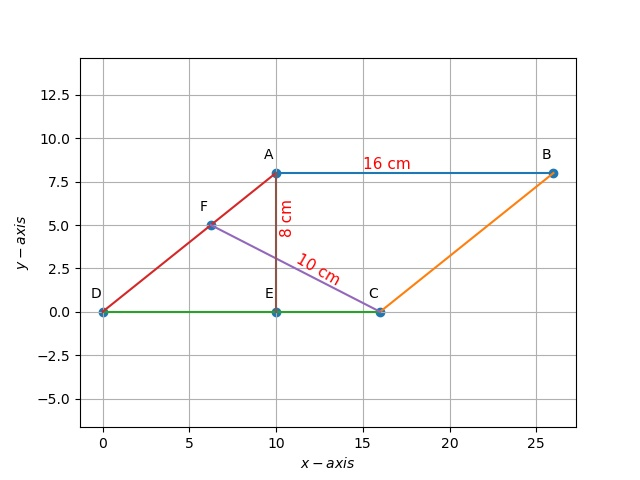
\includegraphics[width=0.5\textwidth]{fig 1.jpeg}
Figure 1 - Parallelogram ABCD


\section{Construction}
\vspace{0.5cm}
\begin{tabular}{|c|c|c|}
\hline
Symbol & Value & Description\\
\hline
D & Origin (0,0) & Vertex D \\
\hline
AB & 16cm & $\|\hspace{0.1cm} \vec{B} - \vec{A} \hspace{0.1cm}\|$ \\
\hline
CD & 16cm & $\|\hspace{0.1cm} \vec{D} - \vec{C} \hspace{0.1cm}\| = \|\hspace{0.1cm} \vec{B} - \vec{A} \hspace{0.1cm}\|$ \\
\hline
C & (16,0) & Vertex C ($\because CD = 16cm$)\\
\hline
AE & 8cm & $\|\hspace{0.1cm} \vec{E} - \vec{A} \hspace{0.1cm}\|$ \\
\hline

\end{tabular}
\begin{tabular}{|c|c|c|}

\hline
CF & 10cm & $\|\hspace{0.1cm} \vec{F} - \vec{C} \hspace{0.1cm}\|$ \\
\hline

A & (10,8) & Ay = Dy + $|\overrightarrow{AE}|$\\
 & & $Ax = \sqrt{\frac{CF^2}{AB^2 - CF^2}}$\\
 
\hline

B & (26,8) & By = Dy + $|\overrightarrow{AE}|$\\
 & & $Bx = Ax + AB$\\
 
\hline
F & (6.25,5) & $Fy = 0.8 \hspace{0.1cm} X\hspace{0.1cm} Fx$\\
\hline

E & (10,0) & Ex = Ax, Ey=0 \\
\hline

\end{tabular}


\section{Solution}
\raggedright
From the properties of Parallelogram we know that, Opposite sides are equal in length. Hence, we can write,\\
\vspace{0.25cm}
\centering
$|\hspace{0.1cm}\overrightarrow{CD}\hspace{0.1cm}| = |\hspace{0.1cm}\overrightarrow{AB}\hspace{0.1cm}|$\\
\vspace{0.25cm}
Hence,
$\|\hspace{0.1cm} \vec{D} - \vec{C} \hspace{0.1cm}\|\hspace{0.1cm} = \hspace{0.1cm} \|\hspace{0.1cm} \vec{B} - \vec{A}\hspace{0.1cm} \|\hspace{0.1cm}=\hspace{0.1cm}16cm$\\
\vspace{0.25cm}
\raggedright
We also know that,\\
\vspace{0.25cm}
\centering
Area of a Parallelogram = Base x Height\\
\vspace{0.25cm}
\raggedright
Since, it is given that $\overrightarrow{AE} \perp \overrightarrow{CD}$  from the figure 1 we can write,\\
\vspace{0.25cm}
Area of Parallelogram ABCD = $|\hspace{0.1cm} \overrightarrow{CD}\hspace{0.1cm}|\hspace{0.1cm} x\hspace{0.1cm}|\hspace{0.1cm}  \overrightarrow{AE}\hspace{0.1cm}|$ \hspace{0.1cm} (1)\\
\vspace{0.25cm}
\hspace{4.5cm} $=\hspace{0.1cm} \|\hspace{0.1cm} \vec{D} - \vec{C} \hspace{0.1cm}\|\hspace{0.1cm} x\hspace{0.1cm} \|\hspace{0.1cm} \vec{E} - \vec{A}\hspace{0.1cm} \|$\\
\vspace{0.25cm}
But it is also given that $\overrightarrow{CF} \perp \overrightarrow{AD}$. Hence we can similarly write,\\
\vspace{0.25cm}
Area of Parallelogram ABCD = $|\hspace{0.1cm} \overrightarrow{AD}\hspace{0.1cm}|\hspace{0.1cm}  x\hspace{0.1cm}|\hspace{0.1cm}  \overrightarrow{CF}\hspace{0.1cm}|$ \hspace{0.1cm} (2)\\
\vspace{0.25cm}
\hspace{4.5cm} $=\hspace{0.1cm} \|\hspace{0.1cm} \vec{D} - \vec{A} \hspace{0.1cm}\|\hspace{0.1cm} x\hspace{0.1cm} \|\hspace{0.1cm} \vec{F} - \vec{C}\hspace{0.1cm} \|$\\
\vspace{0.25cm}
Observing Eq. (1) and Eq. (2), we see that both are equal. Hence we get,\\
\vspace{0.25cm}
\centering

$ \|\hspace{0.1cm} \vec{D} - \vec{C} \hspace{0.1cm}\|\hspace{0.1cm} x\hspace{0.1cm} \|\hspace{0.1cm} \vec{E} - \vec{A}\hspace{0.1cm} \|\hspace{0.1cm} = \hspace{0.1cm} \|\hspace{0.1cm} \vec{D} - \vec{A} \hspace{0.1cm}\|\hspace{0.1cm} x\hspace{0.1cm} \|\hspace{0.1cm} \vec{F} - \vec{C}\hspace{0.1cm} \|  $

\vspace{0.25cm}

$|\hspace{0.1cm} 16\hspace{0.1cm}|\hspace{0.1cm}  x\hspace{0.1cm}|\hspace{0.1cm}  8 \hspace{0.1cm}|= \hspace{0.1cm}  \|\hspace{0.1cm} \vec{D} - \vec{A} \hspace{0.1cm}\| \hspace{0.1cm} x\hspace{0.1cm} |\hspace{0.1cm} 10\hspace{0.1cm}|$\\

\vspace{0.25cm}

128 = $\hspace{0.1cm} \|\hspace{0.1cm} \vec{D} - \vec{A} \hspace{0.1cm}\|\hspace{0.1cm}$ x 10\\

\vspace{0.25cm}

$ \|\hspace{0.1cm} \vec{D} - \vec{A} \hspace{0.1cm}\| \hspace{0.1cm}=\hspace{0.1cm}\frac{128}{10}$\\

\vspace{0.25cm}

$\therefore$ $|\hspace{0.1cm}$\textbf{$\overrightarrow{\vec{AD}}\hspace{0.1cm} |$ = 12.8 cm}\\

\vspace{0.25cm}

\centering
\textbf{Hence, This is the required value of AD.}

\vspace{0.25cm}


\end{document}
Footer